% =============================================================================
% Lecture 4: Trade and Tariffs
% =============================================================================
\documentclass[9pt,english,aspectratio=169]{beamer}
% =============================================================================
% Pathways: Economics & Finance Workshop — Beamer Preamble
% =============================================================================
% Usage: Each lecture .tex file should start with:
%   \documentclass[10pt,english,aspectratio=169]{beamer}
%   % =============================================================================
% Pathways: Economics & Finance Workshop — Beamer Preamble
% =============================================================================
% Usage: Each lecture .tex file should start with:
%   \documentclass[10pt,english,aspectratio=169]{beamer}
%   % =============================================================================
% Pathways: Economics & Finance Workshop — Beamer Preamble
% =============================================================================
% Usage: Each lecture .tex file should start with:
%   \documentclass[10pt,english,aspectratio=169]{beamer}
%   \input{../../codes/Preambles/header_slides}
% Compile: cd output/Slides && TEXINPUTS=../../codes/Preambles:$TEXINPUTS xelatex file.tex
% =============================================================================

% ---------- Packages ----------
% Fonts
\usepackage{lmodern}
\usepackage[utf8]{inputenc}
\usepackage[normalem]{ulem}

% Math
\usepackage{amsmath,amssymb,amsthm}

% Figures and tables
\usepackage{graphicx}
\usepackage{array,tabularx,booktabs,threeparttable}

% TikZ and pgfplots
\usepackage{pgfplots}
\pgfplotsset{compat=1.18}
\usepackage{tikz}
\usetikzlibrary{positioning,arrows.meta,calc}

% Colored boxes
\usepackage[most]{tcolorbox}

% Miscellaneous
\usepackage{transparent}
\usepackage{setspace}
\usepackage[nodayofweek]{datetime}
\usepackage{hyperref}

% ---------- Theme ----------
\usetheme{CambridgeUS}
\usecolortheme{dolphin}
\usepackage{appendixnumberbeamer}

% ---------- Itemize ----------
\setbeamercovered{invisible}
\setbeamertemplate{itemize items}[default]
\setbeamertemplate{enumerate items}[default]

\setbeamertemplate{itemize item}[triangle]
\setbeamertemplate{itemize subitem}[triangle]
\setbeamertemplate{itemize subsubitem}{-}

% ---------- Headline / Footline ----------
\setbeamertemplate{headline}{}

\setbeamertemplate{footline}{
  \leavevmode
  \hbox{
    \begin{beamercolorbox}[wd=\paperwidth,ht=2.5ex,dp=1.25ex,leftskip=1em,rightskip=1em]{footline}
      \hfill \insertframenumber
    \end{beamercolorbox}
  }
}

\setbeamertemplate{navigation symbols}{}

% ---------- Frame title (centered) ----------
\makeatletter
\setbeamertemplate{frametitle}{
  \nointerlineskip
  \begin{beamercolorbox}[wd=\paperwidth,sep=0.35cm,center]{frametitle}
    {\usebeamerfont{frametitle}\insertframetitle\par}
    \ifx\insertframesubtitle\@empty\else
      \vspace{0.15cm}
      {\usebeamerfont{framesubtitle}\usebeamercolor[fg]{framesubtitle}\insertframesubtitle\par}
    \fi
  \end{beamercolorbox}
}
\makeatother

% ---------- Margins ----------
\setbeamersize{
  text margin left=2em,
  text margin right=2em
}

% ---------- Section outline frames ----------
\AtBeginSection[]{
  \begin{frame}{Outline}
    \tableofcontents[currentsection,
                     currentsubsection,
                     hideothersubsections]
  \end{frame}
}

% =============================================================================
% Colors — Okabe-Ito colorblind-friendly palette
% =============================================================================

\definecolor{black}{HTML}{000000}
\definecolor{orange}{HTML}{E69F00}
\definecolor{skyblue}{HTML}{56B4E9}
\definecolor{green}{HTML}{009E73}
\definecolor{yellow}{HTML}{F0E442}
\definecolor{blue}{HTML}{0072B2}
\definecolor{vermillion}{HTML}{D55E00}
\definecolor{purple}{HTML}{CC79A7}

% Semantic aliases (mapped to Okabe-Ito)
\definecolor{softbg}{HTML}{F5F5F5}
\definecolor{lightgray}{gray}{0.65}

% =============================================================================
% Box Environments
% =============================================================================

% --- Key points (orange background) ---
\newtcolorbox{keybox}{
  colback=orange!12,
  colframe=orange,
  fonttitle=\bfseries,
  boxrule=0.5pt,
  arc=2pt,
  left=6pt,
  right=6pt,
  top=4pt,
  bottom=4pt
}

% --- Highlights (orange left accent) ---
\newtcolorbox{highlightbox}{
  colback=white,
  colframe=orange,
  fonttitle=\bfseries,
  boxrule=0pt,
  leftrule=3pt,
  arc=0pt,
  left=6pt,
  right=6pt,
  top=4pt,
  bottom=4pt
}

% --- Definitions (blue border, titled) ---
\newtcolorbox{definitionbox}[1][]{
  colback=blue!5,
  colframe=blue,
  fonttitle=\bfseries,
  title={#1},
  boxrule=0.5pt,
  arc=2pt,
  left=6pt,
  right=6pt,
  top=4pt,
  bottom=4pt
}

% --- Methods (sky blue background) ---
\newtcolorbox{methodbox}{
  colback=skyblue!8,
  colframe=skyblue!70,
  fonttitle=\bfseries,
  boxrule=0.5pt,
  arc=2pt,
  left=6pt,
  right=6pt,
  top=4pt,
  bottom=4pt
}

% --- Results (green border) ---
\newtcolorbox{resultbox}{
  colback=green!5,
  colframe=green,
  fonttitle=\bfseries,
  boxrule=0.5pt,
  arc=2pt,
  left=6pt,
  right=6pt,
  top=4pt,
  bottom=4pt
}

% --- Quotes (purple left rule) ---
\newtcolorbox{quotebox}{
  colback=softbg,
  colframe=purple,
  fonttitle=\itshape,
  boxrule=0pt,
  leftrule=2pt,
  arc=0pt,
  left=6pt,
  right=6pt,
  top=4pt,
  bottom=4pt
}

% =============================================================================
% Math Commands
% =============================================================================

\newcommand{\E}{\mathrm{E}}
\newcommand{\Var}{\mathrm{Var}}
\newcommand{\Cov}{\mathrm{Cov}}
\newcommand{\R}{\mathbb{R}}
\newcommand{\suminfty}[1]{\sum_{#1=0}^\infty}
\newcommand{\Lcal}{\mathcal{L}}
\newcommand{\prtl}[2]{\frac{\partial #1}{\partial #2}}
\renewcommand{\div}[2]{\frac{d #1}{d #2}}
\newcommand{\suchthat}{\text{ s.t. }}
\newcommand{\wrt}{\text{ w.r.t. }}
\newcommand{\red}[1]{\textcolor{vermillion}{#1}}
\newcommand{\blue}[1]{\textcolor{blue}{#1}}

% =============================================================================
% Economics Shortcuts
% =============================================================================

\newcommand{\OC}{\text{Opportunity Cost}}
\newcommand{\DWL}{\text{DWL}}
\newcommand{\pmark}{\textcolor{resultgreen}{\checkmark}}
\newcommand{\xmark}{\textcolor{darkred}{\texttimes}}

% Compile: cd output/Slides && TEXINPUTS=../../codes/Preambles:$TEXINPUTS xelatex file.tex
% =============================================================================

% ---------- Packages ----------
% Fonts
\usepackage{lmodern}
\usepackage[utf8]{inputenc}
\usepackage[normalem]{ulem}

% Math
\usepackage{amsmath,amssymb,amsthm}

% Figures and tables
\usepackage{graphicx}
\usepackage{array,tabularx,booktabs,threeparttable}

% TikZ and pgfplots
\usepackage{pgfplots}
\pgfplotsset{compat=1.18}
\usepackage{tikz}
\usetikzlibrary{positioning,arrows.meta,calc}

% Colored boxes
\usepackage[most]{tcolorbox}

% Miscellaneous
\usepackage{transparent}
\usepackage{setspace}
\usepackage[nodayofweek]{datetime}
\usepackage{hyperref}

% ---------- Theme ----------
\usetheme{CambridgeUS}
\usecolortheme{dolphin}
\usepackage{appendixnumberbeamer}

% ---------- Itemize ----------
\setbeamercovered{invisible}
\setbeamertemplate{itemize items}[default]
\setbeamertemplate{enumerate items}[default]

\setbeamertemplate{itemize item}[triangle]
\setbeamertemplate{itemize subitem}[triangle]
\setbeamertemplate{itemize subsubitem}{-}

% ---------- Headline / Footline ----------
\setbeamertemplate{headline}{}

\setbeamertemplate{footline}{
  \leavevmode
  \hbox{
    \begin{beamercolorbox}[wd=\paperwidth,ht=2.5ex,dp=1.25ex,leftskip=1em,rightskip=1em]{footline}
      \hfill \insertframenumber
    \end{beamercolorbox}
  }
}

\setbeamertemplate{navigation symbols}{}

% ---------- Frame title (centered) ----------
\makeatletter
\setbeamertemplate{frametitle}{
  \nointerlineskip
  \begin{beamercolorbox}[wd=\paperwidth,sep=0.35cm,center]{frametitle}
    {\usebeamerfont{frametitle}\insertframetitle\par}
    \ifx\insertframesubtitle\@empty\else
      \vspace{0.15cm}
      {\usebeamerfont{framesubtitle}\usebeamercolor[fg]{framesubtitle}\insertframesubtitle\par}
    \fi
  \end{beamercolorbox}
}
\makeatother

% ---------- Margins ----------
\setbeamersize{
  text margin left=2em,
  text margin right=2em
}

% ---------- Section outline frames ----------
\AtBeginSection[]{
  \begin{frame}{Outline}
    \tableofcontents[currentsection,
                     currentsubsection,
                     hideothersubsections]
  \end{frame}
}

% =============================================================================
% Colors — Okabe-Ito colorblind-friendly palette
% =============================================================================

\definecolor{black}{HTML}{000000}
\definecolor{orange}{HTML}{E69F00}
\definecolor{skyblue}{HTML}{56B4E9}
\definecolor{green}{HTML}{009E73}
\definecolor{yellow}{HTML}{F0E442}
\definecolor{blue}{HTML}{0072B2}
\definecolor{vermillion}{HTML}{D55E00}
\definecolor{purple}{HTML}{CC79A7}

% Semantic aliases (mapped to Okabe-Ito)
\definecolor{softbg}{HTML}{F5F5F5}
\definecolor{lightgray}{gray}{0.65}

% =============================================================================
% Box Environments
% =============================================================================

% --- Key points (orange background) ---
\newtcolorbox{keybox}{
  colback=orange!12,
  colframe=orange,
  fonttitle=\bfseries,
  boxrule=0.5pt,
  arc=2pt,
  left=6pt,
  right=6pt,
  top=4pt,
  bottom=4pt
}

% --- Highlights (orange left accent) ---
\newtcolorbox{highlightbox}{
  colback=white,
  colframe=orange,
  fonttitle=\bfseries,
  boxrule=0pt,
  leftrule=3pt,
  arc=0pt,
  left=6pt,
  right=6pt,
  top=4pt,
  bottom=4pt
}

% --- Definitions (blue border, titled) ---
\newtcolorbox{definitionbox}[1][]{
  colback=blue!5,
  colframe=blue,
  fonttitle=\bfseries,
  title={#1},
  boxrule=0.5pt,
  arc=2pt,
  left=6pt,
  right=6pt,
  top=4pt,
  bottom=4pt
}

% --- Methods (sky blue background) ---
\newtcolorbox{methodbox}{
  colback=skyblue!8,
  colframe=skyblue!70,
  fonttitle=\bfseries,
  boxrule=0.5pt,
  arc=2pt,
  left=6pt,
  right=6pt,
  top=4pt,
  bottom=4pt
}

% --- Results (green border) ---
\newtcolorbox{resultbox}{
  colback=green!5,
  colframe=green,
  fonttitle=\bfseries,
  boxrule=0.5pt,
  arc=2pt,
  left=6pt,
  right=6pt,
  top=4pt,
  bottom=4pt
}

% --- Quotes (purple left rule) ---
\newtcolorbox{quotebox}{
  colback=softbg,
  colframe=purple,
  fonttitle=\itshape,
  boxrule=0pt,
  leftrule=2pt,
  arc=0pt,
  left=6pt,
  right=6pt,
  top=4pt,
  bottom=4pt
}

% =============================================================================
% Math Commands
% =============================================================================

\newcommand{\E}{\mathrm{E}}
\newcommand{\Var}{\mathrm{Var}}
\newcommand{\Cov}{\mathrm{Cov}}
\newcommand{\R}{\mathbb{R}}
\newcommand{\suminfty}[1]{\sum_{#1=0}^\infty}
\newcommand{\Lcal}{\mathcal{L}}
\newcommand{\prtl}[2]{\frac{\partial #1}{\partial #2}}
\renewcommand{\div}[2]{\frac{d #1}{d #2}}
\newcommand{\suchthat}{\text{ s.t. }}
\newcommand{\wrt}{\text{ w.r.t. }}
\newcommand{\red}[1]{\textcolor{vermillion}{#1}}
\newcommand{\blue}[1]{\textcolor{blue}{#1}}

% =============================================================================
% Economics Shortcuts
% =============================================================================

\newcommand{\OC}{\text{Opportunity Cost}}
\newcommand{\DWL}{\text{DWL}}
\newcommand{\pmark}{\textcolor{resultgreen}{\checkmark}}
\newcommand{\xmark}{\textcolor{darkred}{\texttimes}}

% Compile: cd output/Slides && TEXINPUTS=../../codes/Preambles:$TEXINPUTS xelatex file.tex
% =============================================================================

% ---------- Packages ----------
% Fonts
\usepackage{lmodern}
\usepackage[utf8]{inputenc}
\usepackage[normalem]{ulem}

% Math
\usepackage{amsmath,amssymb,amsthm}

% Figures and tables
\usepackage{graphicx}
\usepackage{array,tabularx,booktabs,threeparttable}

% TikZ and pgfplots
\usepackage{pgfplots}
\pgfplotsset{compat=1.18}
\usepackage{tikz}
\usetikzlibrary{positioning,arrows.meta,calc}

% Colored boxes
\usepackage[most]{tcolorbox}

% Miscellaneous
\usepackage{transparent}
\usepackage{setspace}
\usepackage[nodayofweek]{datetime}
\usepackage{hyperref}

% ---------- Theme ----------
\usetheme{CambridgeUS}
\usecolortheme{dolphin}
\usepackage{appendixnumberbeamer}

% ---------- Itemize ----------
\setbeamercovered{invisible}
\setbeamertemplate{itemize items}[default]
\setbeamertemplate{enumerate items}[default]

\setbeamertemplate{itemize item}[triangle]
\setbeamertemplate{itemize subitem}[triangle]
\setbeamertemplate{itemize subsubitem}{-}

% ---------- Headline / Footline ----------
\setbeamertemplate{headline}{}

\setbeamertemplate{footline}{
  \leavevmode
  \hbox{
    \begin{beamercolorbox}[wd=\paperwidth,ht=2.5ex,dp=1.25ex,leftskip=1em,rightskip=1em]{footline}
      \hfill \insertframenumber
    \end{beamercolorbox}
  }
}

\setbeamertemplate{navigation symbols}{}

% ---------- Frame title (centered) ----------
\makeatletter
\setbeamertemplate{frametitle}{
  \nointerlineskip
  \begin{beamercolorbox}[wd=\paperwidth,sep=0.35cm,center]{frametitle}
    {\usebeamerfont{frametitle}\insertframetitle\par}
    \ifx\insertframesubtitle\@empty\else
      \vspace{0.15cm}
      {\usebeamerfont{framesubtitle}\usebeamercolor[fg]{framesubtitle}\insertframesubtitle\par}
    \fi
  \end{beamercolorbox}
}
\makeatother

% ---------- Margins ----------
\setbeamersize{
  text margin left=2em,
  text margin right=2em
}

% ---------- Section outline frames ----------
\AtBeginSection[]{
  \begin{frame}{Outline}
    \tableofcontents[currentsection,
                     currentsubsection,
                     hideothersubsections]
  \end{frame}
}

% =============================================================================
% Colors — Okabe-Ito colorblind-friendly palette
% =============================================================================

\definecolor{black}{HTML}{000000}
\definecolor{orange}{HTML}{E69F00}
\definecolor{skyblue}{HTML}{56B4E9}
\definecolor{green}{HTML}{009E73}
\definecolor{yellow}{HTML}{F0E442}
\definecolor{blue}{HTML}{0072B2}
\definecolor{vermillion}{HTML}{D55E00}
\definecolor{purple}{HTML}{CC79A7}

% Semantic aliases (mapped to Okabe-Ito)
\definecolor{softbg}{HTML}{F5F5F5}
\definecolor{lightgray}{gray}{0.65}

% =============================================================================
% Box Environments
% =============================================================================

% --- Key points (orange background) ---
\newtcolorbox{keybox}{
  colback=orange!12,
  colframe=orange,
  fonttitle=\bfseries,
  boxrule=0.5pt,
  arc=2pt,
  left=6pt,
  right=6pt,
  top=4pt,
  bottom=4pt
}

% --- Highlights (orange left accent) ---
\newtcolorbox{highlightbox}{
  colback=white,
  colframe=orange,
  fonttitle=\bfseries,
  boxrule=0pt,
  leftrule=3pt,
  arc=0pt,
  left=6pt,
  right=6pt,
  top=4pt,
  bottom=4pt
}

% --- Definitions (blue border, titled) ---
\newtcolorbox{definitionbox}[1][]{
  colback=blue!5,
  colframe=blue,
  fonttitle=\bfseries,
  title={#1},
  boxrule=0.5pt,
  arc=2pt,
  left=6pt,
  right=6pt,
  top=4pt,
  bottom=4pt
}

% --- Methods (sky blue background) ---
\newtcolorbox{methodbox}{
  colback=skyblue!8,
  colframe=skyblue!70,
  fonttitle=\bfseries,
  boxrule=0.5pt,
  arc=2pt,
  left=6pt,
  right=6pt,
  top=4pt,
  bottom=4pt
}

% --- Results (green border) ---
\newtcolorbox{resultbox}{
  colback=green!5,
  colframe=green,
  fonttitle=\bfseries,
  boxrule=0.5pt,
  arc=2pt,
  left=6pt,
  right=6pt,
  top=4pt,
  bottom=4pt
}

% --- Quotes (purple left rule) ---
\newtcolorbox{quotebox}{
  colback=softbg,
  colframe=purple,
  fonttitle=\itshape,
  boxrule=0pt,
  leftrule=2pt,
  arc=0pt,
  left=6pt,
  right=6pt,
  top=4pt,
  bottom=4pt
}

% =============================================================================
% Math Commands
% =============================================================================

\newcommand{\E}{\mathrm{E}}
\newcommand{\Var}{\mathrm{Var}}
\newcommand{\Cov}{\mathrm{Cov}}
\newcommand{\R}{\mathbb{R}}
\newcommand{\suminfty}[1]{\sum_{#1=0}^\infty}
\newcommand{\Lcal}{\mathcal{L}}
\newcommand{\prtl}[2]{\frac{\partial #1}{\partial #2}}
\renewcommand{\div}[2]{\frac{d #1}{d #2}}
\newcommand{\suchthat}{\text{ s.t. }}
\newcommand{\wrt}{\text{ w.r.t. }}
\newcommand{\red}[1]{\textcolor{vermillion}{#1}}
\newcommand{\blue}[1]{\textcolor{blue}{#1}}

% =============================================================================
% Economics Shortcuts
% =============================================================================

\newcommand{\OC}{\text{Opportunity Cost}}
\newcommand{\DWL}{\text{DWL}}
\newcommand{\pmark}{\textcolor{resultgreen}{\checkmark}}
\newcommand{\xmark}{\textcolor{darkred}{\texttimes}}


% ---------- Voting icons ----------
\newcommand{\thumbup}{%
  \begin{tikzpicture}[baseline=-0.3em]
    \fill[green, rounded corners=2pt] (0,0) rectangle (1.4,1.4);
    \node[white, font=\Large\bfseries] at (0.7,0.7) {$\Uparrow$};
  \end{tikzpicture}%
}
\newcommand{\thumbdown}{%
  \begin{tikzpicture}[baseline=-0.3em]
    \fill[vermillion, rounded corners=2pt] (0,0) rectangle (1.4,1.4);
    \node[white, font=\Large\bfseries] at (0.7,0.7) {$\Downarrow$};
  \end{tikzpicture}%
}
\newcommand{\thumbside}{%
  \begin{tikzpicture}[baseline=-0.3em]
    \fill[DarkGray, rounded corners=2pt] (0,0) rectangle (1.4,1.4);
    \node[white, font=\Large\bfseries] at (0.7,0.7) {$\Rightarrow$};
  \end{tikzpicture}%
}

% ---------- Placeholder image handler ----------
\newcommand{\placeholderimg}[2][width=\textwidth]{%
  \IfFileExists{#2}{%
    \includegraphics[#1]{#2}%
  }{%
    \fcolorbox{gray!30}{gray!10}{\parbox{3.8cm}{\centering\vspace{0.8cm}{\tiny\itshape\textcolor{gray}{placeholder}}\vspace{0.8cm}}}%
  }%
}

% ---------- Title ----------
\title{\textbf{Trade and Tariffs}}
\subtitle{Pathways to Arts \& Humanities Summer Scholars Program}
\author{Instructor: Tudor Schlanger}
\date{Summer 2026}

\begin{document}

% =============================================================================
% Title
% =============================================================================
\begin{frame}
  \titlepage
\end{frame}

% =============================================================================
% Review
% =============================================================================

\begin{frame}{Review: Tragedy of the Commons}

  \begin{questionbox}
    A town has a public lake where anyone can fish for free.
    Over time, the fish population declines sharply.

    \vspace{0.5em}
    Which combination of properties makes the fish a \textbf{common resource}?
  \end{questionbox}

  \vspace{0.6em}
  \begin{enumerate}[A.]
    \item Rivalrous and excludable
    \item Non-rivalrous and non-excludable
    \item Rivalrous and non-excludable
    \item Non-rivalrous and excludable
  \end{enumerate}

\end{frame}

\begin{frame}{Review: Tragedy of the Commons --- Answer}

  \begin{answerbox}
    The correct answer is \textbf{C. Rivalrous and non-excludable}.\\[0.5em]
    The fish are \textbf{rivalrous}: one person's catch reduces what is available for others.\\[0.3em]
    The lake is \textbf{non-excludable}: anyone can fish without paying.\\[0.3em]
    This combination creates the Tragedy of the Commons --- overfishing depletes the resource.
  \end{answerbox}

\end{frame}

% =============================================================================
% Opening Quiz
% =============================================================================

\begin{frame}{Claim 1}
  \centering

  {\Large\textbf{``International trade is generally good for a country's economy.''}}

  \vspace{2em}
  \thumbup\hspace{2em}
  \thumbdown\hspace{2em}
  \thumbside\\[0.5em]
  \textcolor{green}{\textbf{Agree}} \hspace{2.5em}
  \textcolor{vermillion}{\textbf{Disagree}} \hspace{2em}
  \textcolor{DarkGray}{\textbf{Not sure}}

\end{frame}

\begin{frame}{Claim 2}
  \centering

  {\Large\textbf{``International trade is generally good for \underline{every sector} of a country's economy.''}}

  \vspace{2em}
  \thumbup\hspace{2em}
  \thumbdown\hspace{2em}
  \thumbside\\[0.5em]
  \textcolor{green}{\textbf{Agree}} \hspace{2.5em}
  \textcolor{vermillion}{\textbf{Disagree}} \hspace{2em}
  \textcolor{DarkGray}{\textbf{Not sure}}

\end{frame}

\begin{frame}{Claim 3}
  \centering

  {\Large\textbf{``If international trade is not good for every sector, \underline{tariffs} can protect those affected sectors.''}}

  \vspace{2em}
  \thumbup\hspace{2em}
  \thumbdown\hspace{2em}
  \thumbside\\[0.5em]
  \textcolor{green}{\textbf{Agree}} \hspace{2.5em}
  \textcolor{vermillion}{\textbf{Disagree}} \hspace{2em}
  \textcolor{DarkGray}{\textbf{Not sure}}

  \vspace{1.5em}
  \textcolor{DarkGray}{\textit{We'll revisit these at the end of class.}}

\end{frame}

% =============================================================================
\section{Is Trade Good for a Country?}
% =============================================================================

\begin{frame}{What Is International Trade?}

  \begin{columns}[T]
    \begin{column}{0.58\textwidth}
      \begin{definitionbox}[International Trade]
        The exchange of goods and services across national borders.
      \end{definitionbox}

      \vspace{1.5em}
      \textcolor{purple}{\textbf{Imports}} = goods coming IN to a country
      {\small\textit{\textcolor{DarkGray}{(your phone, made in China, imported to the U.S.)}}}

      \vspace{0.8em}
      \textcolor{green}{\textbf{Exports}} = goods going OUT of a country
      {\small\textit{\textcolor{DarkGray}{(U.S.\ soybeans, shipped to China)}}}
    \end{column}
    \begin{column}{0.38\textwidth}
      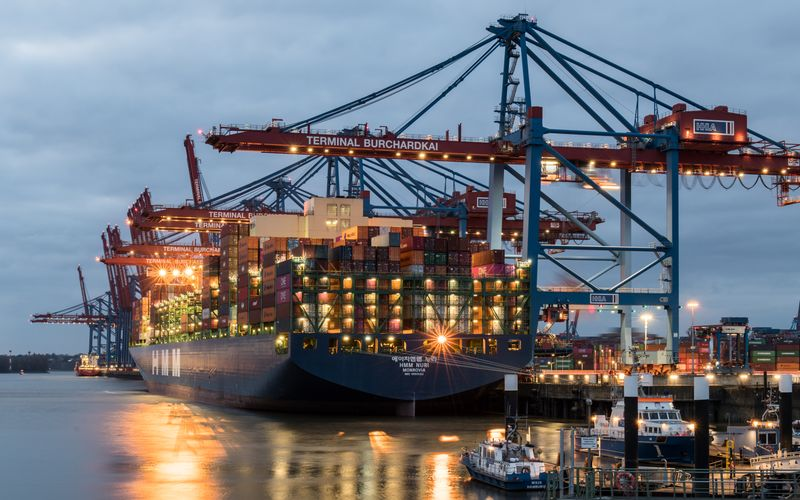
\includegraphics[width=\textwidth]{fig/container_ship_port.jpg}
    \end{column}
  \end{columns}

\end{frame}

\begin{frame}{Why Do Countries Trade?}

  \begin{columns}[T]
    \begin{column}{0.58\textwidth}
      \vspace{0.5em}
      Not every country can make everything well:

      \vspace{0.8em}
      \begin{itemize}
        \item Different climates, resources, and skills
        \item Some countries have more workers; others have more technology
        \item Making everything yourself is expensive and slow
      \end{itemize}
    \end{column}
    \begin{column}{0.38\textwidth}
      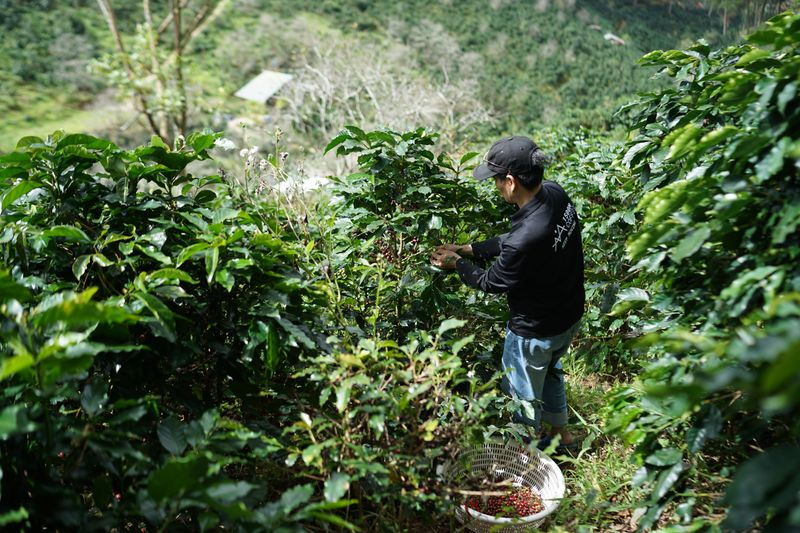
\includegraphics[width=\textwidth, height=0.35\textheight, keepaspectratio]{fig/coffee_plantation.jpg}

      \vspace{0.5em}
      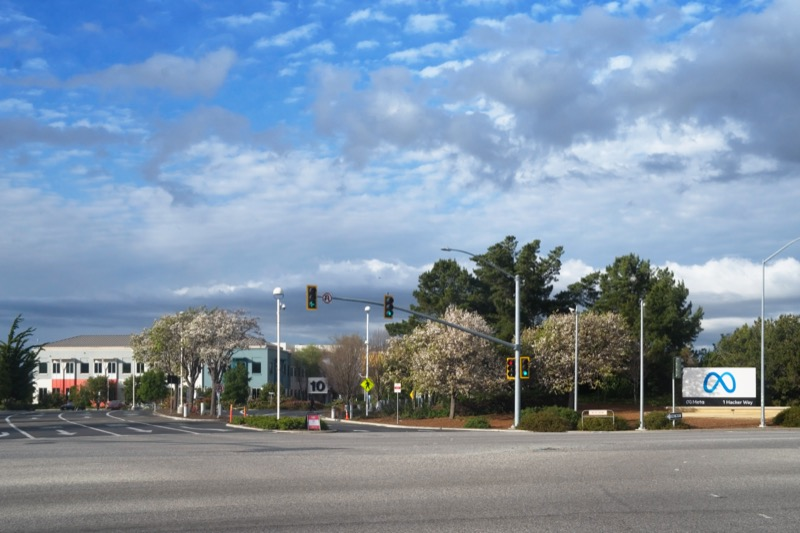
\includegraphics[width=\textwidth, height=0.35\textheight, keepaspectratio]{fig/meta_hq.jpg}
    \end{column}
  \end{columns}

\end{frame}

% ---------- Comparative Advantage Example ----------

\begin{frame}{A Tale of Two Countries}

  \begin{questionbox}
    Imagine a country that \textit{is} good at everything. Should it trade at all?
  \end{questionbox}

  \pause
  \vspace{0.8em}
  \begin{columns}[T]
    \begin{column}{0.48\textwidth}
      \textbf{The setup:} Each country has 100 workers.

      \vspace{1.2em}
      \textcolor{blue}{\textbf{United States}}\\
      Good at producing both software AND coffee\\
      {\small Especially productive at software}

      \vspace{1.2em}
      \textcolor{orange}{\textbf{Colombia}}\\
      Less productive at both\\
      {\small But relatively better at coffee} \pause
    \end{column}
    \begin{column}{0.48\textwidth}
      \vspace{0.5em}
      {\small With 100 workers, each can produce:}

      \vspace{0.8em}
      \begin{tabular}{@{} l c c @{}}
        \toprule
        & \textbf{Software} & \textbf{Coffee} \\
        & (units) & (tons) \\
        \midrule
        \textcolor{blue}{\textbf{U.S.}} & 40 & 20 \\
        \textcolor{orange}{\textbf{Colombia}} & 10 & 20 \\
        \bottomrule
      \end{tabular}

    \end{column}
  \end{columns}

\end{frame}

\begin{frame}{The Key: Opportunity Cost}

  \begin{definitionbox}[Opportunity Cost (OC)]
    The \textbf{value} of the \textbf{next best alternative} when you make a decision.
  \end{definitionbox}

  \vspace{1em}
  \centering
  {\small With 100 workers, each can produce:}

  \vspace{0.8em}
  \begin{tabular}{@{} l c c c c @{}}
    \toprule
    & \textbf{Software} & \textbf{Coffee} & \textbf{OC of Coffee} & \textbf{Benefit/OC} \\
    & (units) & (tons) & (software units) & (units/ton) \\
    \midrule
    \textcolor{blue}{\textbf{U.S.}} & 40 & 20 & & \\
    \textcolor{orange}{\textbf{Colombia}} & 10 & 20 & & \\
    \bottomrule
  \end{tabular}

\end{frame}

\begin{frame}{The Key: Opportunity Cost}

  \begin{definitionbox}[Opportunity Cost (OC)]
    The \textbf{value} of the \textbf{next best alternative} when you make a decision.
  \end{definitionbox}

  \vspace{1em}
  \centering
  {\small With 100 workers, each can produce:}

  \vspace{0.8em}
  \begin{tabular}{@{} l c c c c @{}}
    \toprule
    & \textbf{Software} & \textbf{Coffee} & \textbf{OC of Coffee} & \textbf{Benefit/OC} \\
    & (units) & (tons) & (software units) & (units/ton) \\
    \midrule
    \textcolor{blue}{\textbf{U.S.}} & 40 & 20 & 40 & \\
    \textcolor{orange}{\textbf{Colombia}} & 10 & 20 & 10 & \\
    \bottomrule
  \end{tabular}

  \vspace{0.8em}
  If the U.S.\ shifts all 100 workers to coffee, it gives up \textbf{40 software units} to get 20 tons of coffee. So the OC of coffee = 40 software units. Similarly, Colombia gives up \textbf{10 software units}.

\end{frame}

\begin{frame}{The Key: Opportunity Cost}

  \begin{definitionbox}[Opportunity Cost (OC)]
    The \textbf{value} of the \textbf{next best alternative} when you make a decision.
  \end{definitionbox}

  \vspace{1em}
  \centering
  {\small With 100 workers, each can produce:}

  \vspace{0.8em}
  \begin{tabular}{@{} l c c c c @{}}
    \toprule
    & \textbf{Software} & \textbf{Coffee} & \textbf{OC of Coffee} & \textbf{Benefit/OC} \\
    & (units) & (tons) & (software units) & (units/ton) \\
    \midrule
    \textcolor{blue}{\textbf{U.S.}} & 40 & 20 & 40 & $\frac{1}{2}$ \\
    \textcolor{orange}{\textbf{Colombia}} & 10 & 20 & 10 & 2 \\
    \bottomrule
  \end{tabular}

  \vspace{0.8em}
  Benefit/OC = Coffee / OC of Coffee. Colombia gets \textbf{2 tons per software unit} sacrificed, while the U.S.\ gets only $\frac{1}{2}$. Coffee is a much better deal for Colombia!

    \pause 
    
  \vspace{0.5em}
  \begin{insightbox}
    The Benefit / Opportunity Cost ratio of producing Coffee is much higher for Colombia than it is for the US!
  \end{insightbox}

\end{frame}

\begin{frame}{Absolute Advantage}

  \begin{definitionbox}[Absolute Advantage]
    Being the \textbf{most productive} at producing a good---making more of it with the same resources.
  \end{definitionbox}

  \vspace{1.5em}
  \centering
  \begin{tabular}{@{} l c @{}}
    \toprule
    & \textbf{Absolute Advantage} \\
    & {\small (most productive)} \\
    \midrule
    \textcolor{blue}{\textbf{United States}} & Software \& Coffee \\[0.3em]
    \textcolor{orange}{\textbf{Colombia}} & --- \\
    \bottomrule
  \end{tabular}

  \vspace{1.5em}
  The U.S.\ can produce \textbf{at least as many} goods with the same number of workers. So should it even bother trading?

\end{frame}

\begin{frame}{Comparative Advantage}

  \begin{definitionbox}[Comparative Advantage]
    Being \textbf{relatively better} at producing something, i.e.\ having a higher benefit / opportunity cost ratio.
  \end{definitionbox}

  \vspace{1.5em}
  \centering
  \begin{tabular}{@{} l c c @{}}
    \toprule
    & \textbf{Absolute Advantage} & \textbf{Comparative Advantage} \\
    & {\small (most productive)} & {\small (highest Benefit/OC)} \\
    \midrule
    \textcolor{blue}{\textbf{United States}} & Software \& Coffee & Software \\[0.3em]
    \textcolor{orange}{\textbf{Colombia}} & --- & Coffee \\
    \bottomrule
  \end{tabular}

  \vspace{1.5em}
  The U.S.\ is more productive at \textbf{both} goods (absolute advantage), but each country has a comparative advantage in the good where its Benefit/OC is highest.

\end{frame}

\begin{frame}{No Trade: Each Country Makes Everything}

  \vspace{0.5em}
  If each country splits its workers 50/50 between software and coffee, then the countries would produce:

  \vspace{1em}
  \centering
  \begin{tabular}{@{} l c c @{}}
    \toprule
    & \textbf{Software (units)} & \textbf{Coffee (tons)} \\
    \midrule
    \textcolor{blue}{\textbf{United States}} & 20 & 10 \\
    \textcolor{orange}{\textbf{Colombia}} & 5 & 10 \\
    \midrule
    \textbf{World total} & 25 & 20 \\
    \bottomrule
  \end{tabular}

  \vspace{1.5em}
  \textcolor{DarkGray}{\textit{Not bad---but can they do better?}}

\end{frame}

\begin{frame}{With Trade: Specialize and Swap}

  \begin{columns}[T]
    \begin{column}{0.48\textwidth}
      \textbf{Step 1: Specialize}

      \vspace{0.5em}
      Each country puts all workers on its comparative advantage:

      \vspace{0.8em}
      \centering
      \begin{tabular}{@{} l c c @{}}
        \toprule
        & \textbf{Software} & \textbf{Coffee} \\
        & (units) & (tons) \\
        \midrule
        \textcolor{blue}{\textbf{U.S.}} & 40 & 0 \\
        \textcolor{orange}{\textbf{Colombia}} & 0 & 20 \\
        \bottomrule
      \end{tabular}
    \end{column}
    \begin{column}{0.48\textwidth}
      \pause
      \textbf{Step 2: Trade}

      \vspace{0.5em}
      The U.S.\ gives Colombia 10 software units for 10 tons of coffee.

      \vspace{0.8em}
      \centering
      \begin{tabular}{@{} l c c @{}}
        \toprule
        & \textbf{Software} & \textbf{Coffee} \\
        & (units) & (tons) \\
        \midrule
        \textcolor{blue}{\textbf{U.S.}} & 30 & 10 \\
        \textcolor{orange}{\textbf{Colombia}} & 10 & 10 \\
        \bottomrule
      \end{tabular}
    \end{column}
  \end{columns}

\end{frame}

\begin{frame}{Gains from Trade}

  \begin{columns}[T]
    \begin{column}{0.48\textwidth}
      \red{\textbf{No Trade}} {\small (50/50 split)}

      \vspace{0.8em}
      \centering
      \begin{tabular}{@{} l c c @{}}
        \toprule
        & \textbf{Software} & \textbf{Coffee} \\
        & (units) & (tons) \\
        \midrule
        \textcolor{blue}{\textbf{U.S.}} & 20 & 10 \\
        \textcolor{orange}{\textbf{Colombia}} & 5 & 10 \\
        \midrule
        \textbf{World} & 25 & 20 \\
        \bottomrule
      \end{tabular}
    \end{column}
    \begin{column}{0.48\textwidth}
      \green{\textbf{With Trade}} {\small (specialize + swap)}

      \vspace{0.8em}
      \centering
      \begin{tabular}{@{} l c c @{}}
        \toprule
        & \textbf{Software} & \textbf{Coffee} \\
        & (units) & (tons) \\
        \midrule
        \textcolor{blue}{\textbf{U.S.}} & 30 & 10 \\
        \textcolor{orange}{\textbf{Colombia}} & 10 & 10 \\
        \midrule
        \textbf{World} & 40 & 20 \\
        \bottomrule
      \end{tabular}
    \end{column}
  \end{columns}

  \vspace{1.5em}
  \pause
  \begin{insightbox}
    Same coffee, but \textbf{15 more software units} for the world.
    The U.S.\ gains +10, Colombia gains +5. \textcolor{green}{\textbf{Both countries are better off!}}
  \end{insightbox}

  \vspace{0.8em}
  \textcolor{DarkGray}{\textit{Even though the U.S.\ is more productive at \textbf{both} goods, trade still
  helps---each country specializes in what it does \textit{relatively} best.}}

\end{frame}

\begin{frame}{Claim 1: Is Trade Good for a Country?}
  \centering

  {\Large\textbf{``International trade is generally good for a country's economy.''}}

  \vspace{2em}
  \pause
  \begin{answerbox}
    \textbf{Yes}---international trade generally grows the economic pie.
    Through specialization and comparative advantage, countries produce more
    together than they could alone.
  \end{answerbox}

\end{frame}

% =============================================================================
\section{Does Everyone Benefit?}
% =============================================================================

\begin{frame}{A Bigger Pie, But Who Gets the Slices?}

  \begin{columns}[T]
    \begin{column}{0.48\textwidth}
      \red{\textbf{No Trade}} {\small (50/50 split)}

      \vspace{0.8em}
      \centering
      \begin{tabular}{@{} l c c @{}}
        \toprule
        & \textbf{Software} & \textbf{Coffee} \\
        & (units) & (tons) \\
        \midrule
        \textcolor{blue}{\textbf{U.S.}} & 20 & 10 \\
        \textcolor{orange}{\textbf{Colombia}} & 5 & 10 \\
        \midrule
        \textbf{World} & 25 & 20 \\
        \bottomrule
      \end{tabular}
    \end{column}
    \begin{column}{0.48\textwidth}
      \green{\textbf{Full Specialization}}

      \vspace{0.8em}
      \centering
      \begin{tabular}{@{} l c c @{}}
        \toprule
        & \textbf{Software} & \textbf{Coffee} \\
        & (units) & (tons) \\
        \midrule
        \textcolor{blue}{\textbf{U.S.}} & 40 & 0 \\
        \textcolor{orange}{\textbf{Colombia}} & 0 & 20 \\
        \midrule
        \textbf{World} & 40 & 20 \\
        \bottomrule
      \end{tabular}
    \end{column}
  \end{columns}

  \vspace{1em}
  \textbf{Assumption:} Workers can be moved from one sector to another \textbf{without any cost}.

  \pause
  \begin{questionbox}
    What is the problem with this assumption?
  \end{questionbox}

\end{frame}

\begin{frame}{Costs of Specialization}

  \begin{questionbox}
    What is the problem with this assumption?
  \end{questionbox}

  \vspace{0.8em}
  \begin{answerbox}
      \begin{itemize}
      \item Workers in shrinking sectors \textbf{lose their jobs} in the short run
      \item They need to be \textbf{retrained} for a new job, which takes time and money
      \item If the new job requires higher skills, they may also need a \textbf{college education}
      \item If the new job is in a different city, they need to be \textbf{highly mobile}, i.e. willing and able to relocate
    \end{itemize}
  \end{answerbox}

\end{frame}

\begin{frame}{Deindustrialization in America}

  \centering
  \begin{tikzpicture}
    \pgfplotsset{
      every axis/.style={
        width=0.88\textwidth,
        height=6.5cm,
        xmin=1986, xmax=2008,
        xtick={1987,1989,...,2007},
        xticklabel style={font=\tiny, /pgf/number format/1000 sep={}},
        grid=major,
        grid style={gray!20},
        xlabel style={font=\small},
      }
    }
    % Left axis: Import Competition
    \begin{axis}[
      axis y line*=left,
      xlabel={Year},
      ylabel={\textcolor{blue}{Import Competition}},
      ylabel style={font=\small},
      ymin=0, ymax=0.06,
      ytick={0, 0.01, 0.02, 0.03, 0.04, 0.05, 0.06},
      yticklabel style={font=\tiny, color=blue},
    ]
      \addplot[blue, thick, mark=none, smooth] coordinates {
        (1987,0.002) (1988,0.003) (1989,0.004) (1990,0.005)
        (1991,0.006) (1992,0.008) (1993,0.009) (1994,0.010)
        (1995,0.011) (1996,0.012) (1997,0.013) (1998,0.015)
        (1999,0.017) (2000,0.020) (2001,0.021) (2002,0.024)
        (2003,0.028) (2004,0.032) (2005,0.035) (2006,0.040)
        (2007,0.045)
      };
    \end{axis}
    % Right axis: Manufacturing employment / population
    \begin{axis}[
      axis y line*=right,
      axis x line=none,
      ylabel={\textcolor{vermillion}{Manuf.\ emp / population}},
      ylabel style={font=\small},
      ymin=0.08, ymax=0.14,
      ytick={0.08, 0.09, 0.10, 0.11, 0.12, 0.13, 0.14},
      yticklabel style={font=\tiny, color=vermillion},
      xmin=1986, xmax=2008,
    ]
      \addplot[vermillion, thick, dashed, mark=none, smooth] coordinates {
        (1987,0.133) (1988,0.132) (1989,0.130) (1990,0.125)
        (1991,0.120) (1992,0.118) (1993,0.117) (1994,0.119)
        (1995,0.120) (1996,0.119) (1997,0.119) (1998,0.117)
        (1999,0.115) (2000,0.110) (2001,0.100) (2002,0.095)
        (2003,0.093) (2004,0.091) (2005,0.090) (2006,0.088)
        (2007,0.085)
      };
    \end{axis}
  \end{tikzpicture}

  \vspace{0.3em}
  {\tiny\textcolor{lightgray}{Source: Autor, Dorn \& Hanson (2013), Figure 1}}

\end{frame}

\begin{frame}{The China Shock}

  \vspace{0.3em}
  Economists studied what happened to U.S.\ communities most exposed to Chinese imports (Autor, Dorn \& Hanson 2021 BPEA)

  \vspace{0.5em}
  \begin{columns}[T]
    \begin{column}{0.45\textwidth}
      \begin{itemize}
        \item China's entry to the WTO (2001) flooded the U.S.\ with cheap manufactured goods

        \vspace{0.4em}
        \item Regions most exposed saw persistent \textbf{job losses} in manufacturing, \textbf{lower income per capita}

        \vspace{0.4em}
        \item Net out-migration only for foreign-born workers and young native born 
      \end{itemize}
    \end{column}
    \begin{column}{0.54\textwidth}
      \centering
      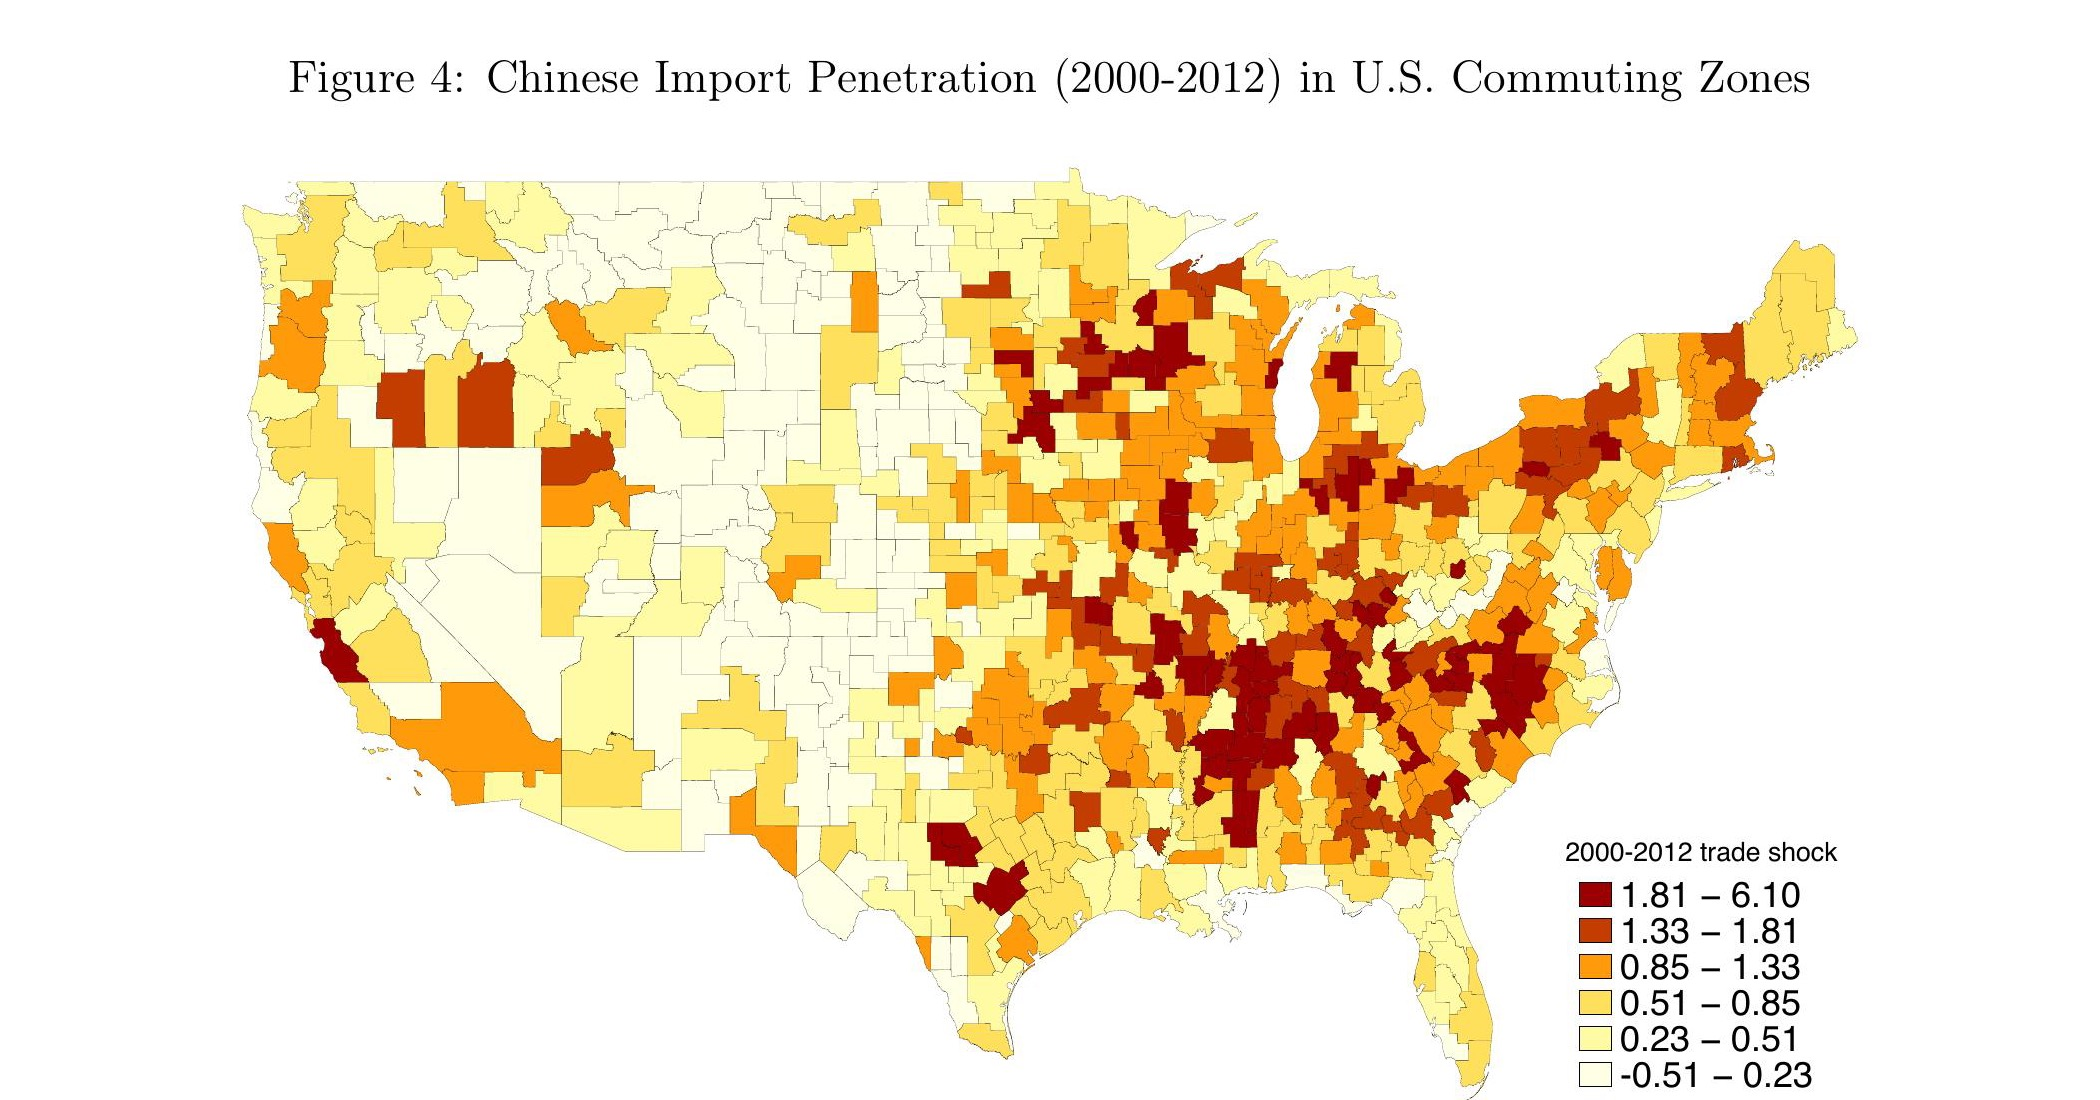
\includegraphics[width=\textwidth]{fig/china_shock_map.jpg}

      \vspace{0.3em}
      {\tiny\textcolor{lightgray}{Source: Autor, Dorn \& Hanson (2021), Figure 4}}
    \end{column}
  \end{columns}

\end{frame}


\begin{frame}{Claim 2: Does Every Sector Benefit?}
  \centering

  {\Large\textbf{``International trade is generally good for \underline{every sector} of a country's economy.''}}

  \vspace{2em}
  \pause
  \begin{answerbox}
    \textbf{No}---not every sector benefits from trade. Trade creates winners
    and losers. Import-competing industries shrink, and workers in those sectors
    face persistent job losses. Transition to growing sectors is possible in
    theory, but difficult, slow, and painful in practice.
  \end{answerbox}

\end{frame}

% =============================================================================
\section{Are Tariffs the Answer?}
% =============================================================================

\begin{frame}{What Is a Tariff?}

  \begin{definitionbox}[Tariff]
    A tax on \underline{imported} goods, paid at the border by the importing firm.
  \end{definitionbox}

  \pause
\vspace{0.5em}
  \begin{tikzpicture}[
    node distance=2.2cm,
    box/.style={draw=DarkGray, rounded corners=3pt, minimum height=1.6cm,
                minimum width=2.8cm, text width=2.6cm, align=center,
                font=\small},
    arr/.style={-{Stealth[length=3mm]}, thick, DarkGray}
  ]
    % Nodes
    \node[box] (foreign) {{\normalsize\textcolor{skyblue}{\textbf{EXPORTER}}}\\[2pt]Chinese firm\\exports the TV};
    \node[box, right=of foreign] (importer) {{\normalsize\textcolor{orange}{\textbf{IMPORTER}}}\\[2pt]Best Buy\\imports the TV};
    \node[box, right=of importer] (consumer) {{\normalsize\textcolor{green}{\textbf{CONSUMER}}}\\[2pt]U.S.\ customers\\buy the TV};

    % Arrows
    \draw[arr] (foreign) -- (importer);
    \draw[arr] (importer) -- (consumer);

    % Tariff annotation
    \node[fill=vermillion!15, draw=vermillion, rounded corners=2pt,
          font=\footnotesize\bfseries, text=vermillion,
          above=0.6cm of importer] (tariff)
          {Tariff imposed at the customs};
    \draw[-{Stealth}, vermillion, thick] (tariff) -- (importer);

  \end{tikzpicture}

\end{frame}

\begin{frame}{Who Bears the Cost of the Tariff?}

  \textbf{Base case:} Small tariff. 

  \vspace{1.5em}
  \centering
  \begin{tikzpicture}[xscale=0.85]
    % Bar dimensions: total width = 13cm, height = 1.2cm
    % $100 cost = 10cm, $10 tariff = 1cm, $20 margin = 2cm
    \def\barh{1.2}

    % Cost of Chinese good ($100)
    \fill[skyblue!60] (0,0) rectangle (10,\barh);
    \node[font=\small\bfseries, anchor=center] at (5,\barh/2) {Cost of Chinese good: \$100};

    % Tariff paid by importer ($10)
    \fill[vermillion!60] (10,0) rectangle (11,\barh);
    \node[font=\tiny\bfseries, anchor=center, text width=1cm, align=center] at (10.5,\barh/2) {Tariff \$10};

    % Margin of the importer ($20)
    \fill[orange!50] (11,0) rectangle (13,\barh);
    \node[font=\small\bfseries, anchor=center] at (12,\barh/2) {Margin: \$20};

    % Borders
    \draw[black, thick] (0,0) rectangle (13,\barh);
    \draw[black] (10,0) -- (10,\barh);
    \draw[black] (11,0) -- (11,\barh);

    % Price label on the right
    \draw[thick, -{Stealth}] (13.3,\barh/2) -- (13.8,\barh/2);
    \node[font=\normalsize\bfseries, anchor=west, text=green] at (13.9,\barh/2) {\$130};

    % === Second bar: higher tariff ($20), Chinese cost drops to $90 ===
    \def\baroffset{-2.2}
    \node[font=\normalsize\bfseries, anchor=south west] at (0,\baroffset+\barh+0.1) {Option A --- Extra tariff paid by the \blue{exporter}:};

    % Cost of Chinese good ($90)
    \fill[skyblue!60] (0,\baroffset) rectangle (9,\baroffset+\barh);
    \node[font=\small\bfseries, anchor=center] at (4.5,\baroffset+\barh/2) {Cost of Chinese good: \$90};

    % Tariff paid by importer ($20)
    \fill[vermillion!60] (9,\baroffset) rectangle (11,\baroffset+\barh);
    \node[font=\small\bfseries, anchor=center] at (10,\baroffset+\barh/2) {Tariff: \$20};

    % Margin of the importer ($20)
    \fill[orange!50] (11,\baroffset) rectangle (13,\baroffset+\barh);
    \node[font=\small\bfseries, anchor=center] at (12,\baroffset+\barh/2) {Margin: \$20};

    % Borders
    \draw[black, thick] (0,\baroffset) rectangle (13,\baroffset+\barh);
    \draw[black] (9,\baroffset) -- (9,\baroffset+\barh);
    \draw[black] (11,\baroffset) -- (11,\baroffset+\barh);

    % Price label on the right
    \draw[thick, -{Stealth}] (13.3,\baroffset+\barh/2) -- (13.8,\baroffset+\barh/2);
    \node[font=\normalsize\bfseries, anchor=west, text=green] at (13.9,\baroffset+\barh/2) {\$130};

    % Invisible anchor to match width of third slide
    \path (15.5,0);

  \end{tikzpicture}

\end{frame}

\begin{frame}{Who Bears the Cost of the Tariff?}

  \textbf{Base case:} Small tariff.

  \vspace{1.5em}
  \centering
  \begin{tikzpicture}[xscale=0.85]
    \def\barh{1.2}

    % Cost of Chinese good ($100)
    \fill[skyblue!60] (0,0) rectangle (10,\barh);
    \node[font=\small\bfseries, anchor=center] at (5,\barh/2) {Cost of Chinese good: \$100};

    % Tariff paid by importer ($10)
    \fill[vermillion!60] (10,0) rectangle (11,\barh);
    \node[font=\tiny\bfseries, anchor=center, text width=1cm, align=center] at (10.5,\barh/2) {Tariff \$10};

    % Margin of the importer ($20)
    \fill[orange!50] (11,0) rectangle (13,\barh);
    \node[font=\small\bfseries, anchor=center] at (12,\barh/2) {Margin: \$20};

    % Borders
    \draw[black, thick] (0,0) rectangle (13,\barh);
    \draw[black] (10,0) -- (10,\barh);
    \draw[black] (11,0) -- (11,\barh);

    % Price label on the right
    \draw[thick, -{Stealth}] (13.3,\barh/2) -- (13.8,\barh/2);
    \node[font=\normalsize\bfseries, anchor=west, text=green] at (13.9,\barh/2) {\$130};

    % === Second bar: tariff paid by importer ===
    \def\baroffset{-2.2}
    \node[font=\normalsize\bfseries, anchor=south west] at (0,\baroffset+\barh+0.1) {Option B --- Extra tariff paid by the \textcolor{vermillion}{importer}:};

    % Cost of Chinese good ($100)
    \fill[skyblue!60] (0,\baroffset) rectangle (10,\baroffset+\barh);
    \node[font=\small\bfseries, anchor=center] at (5,\baroffset+\barh/2) {Cost of Chinese good: \$100};

    % Tariff paid by importer ($20)
    \fill[vermillion!60] (10,\baroffset) rectangle (12,\baroffset+\barh);
    \node[font=\small\bfseries, anchor=center] at (11,\baroffset+\barh/2) {Tariff: \$20};

    % Margin of the importer ($10)
    \fill[orange!50] (12,\baroffset) rectangle (13,\baroffset+\barh);
    \node[font=\tiny\bfseries, anchor=center, text width=1cm, align=center] at (12.5,\baroffset+\barh/2) {Margin \$10};

    % Borders
    \draw[black, thick] (0,\baroffset) rectangle (13,\baroffset+\barh);
    \draw[black] (10,\baroffset) -- (10,\baroffset+\barh);
    \draw[black] (12,\baroffset) -- (12,\baroffset+\barh);

    % Price label on the right
    \draw[thick, -{Stealth}] (13.3,\baroffset+\barh/2) -- (13.8,\baroffset+\barh/2);
    \node[font=\normalsize\bfseries, anchor=west, text=green] at (13.9,\baroffset+\barh/2) {\$130};

    % Invisible anchor to match width of third slide
    \path (15.5,0);

  \end{tikzpicture}

\end{frame}

\begin{frame}{Who Bears the Cost of the Tariff?}

  \textbf{Base case:} Small tariff.

  \vspace{1.5em}
  \centering
  \begin{tikzpicture}[xscale=0.85]
    \def\barh{1.2}

    % Cost of Chinese good ($100)
    \fill[skyblue!60] (0,0) rectangle (10,\barh);
    \node[font=\small\bfseries, anchor=center] at (5,\barh/2) {Cost of Chinese good: \$100};

    % Tariff paid by importer ($10)
    \fill[vermillion!60] (10,0) rectangle (11,\barh);
    \node[font=\tiny\bfseries, anchor=center, text width=1cm, align=center] at (10.5,\barh/2) {Tariff \$10};

    % Margin of the importer ($20)
    \fill[orange!50] (11,0) rectangle (13,\barh);
    \node[font=\small\bfseries, anchor=center] at (12,\barh/2) {Margin: \$20};

    % Borders
    \draw[black, thick] (0,0) rectangle (13,\barh);
    \draw[black] (10,0) -- (10,\barh);
    \draw[black] (11,0) -- (11,\barh);

    % Price label on the right
    \draw[thick, -{Stealth}] (13.3,\barh/2) -- (13.8,\barh/2);
    \node[font=\normalsize\bfseries, anchor=west, text=green] at (13.9,\barh/2) {\$130};

    % === Second bar: tariff paid by consumer (bar extends to $140) ===
    \def\baroffset{-2.2}
    \node[font=\normalsize\bfseries, anchor=south west] at (0,\baroffset+\barh+0.1) {Option C --- Extra tariff paid by the \green{consumer}:};

    % Cost of Chinese good ($100)
    \fill[skyblue!60] (0,\baroffset) rectangle (10,\baroffset+\barh);
    \node[font=\small\bfseries, anchor=center] at (5,\baroffset+\barh/2) {Cost of Chinese good: \$100};

    % Tariff ($20)
    \fill[vermillion!60] (10,\baroffset) rectangle (12,\baroffset+\barh);
    \node[font=\small\bfseries, anchor=center] at (11,\baroffset+\barh/2) {Tariff: \$20};

    % Margin of the importer ($20)
    \fill[orange!50] (12,\baroffset) rectangle (14,\baroffset+\barh);
    \node[font=\small\bfseries, anchor=center] at (13,\baroffset+\barh/2) {Margin: \$20};

    % Borders
    \draw[black, thick] (0,\baroffset) rectangle (14,\baroffset+\barh);
    \draw[black] (10,\baroffset) -- (10,\baroffset+\barh);
    \draw[black] (12,\baroffset) -- (12,\baroffset+\barh);

    % Price label on the right
    \draw[thick, -{Stealth}] (14.3,\baroffset+\barh/2) -- (14.8,\baroffset+\barh/2);
    \node[font=\normalsize\bfseries, anchor=west, text=vermillion] at (14.9,\baroffset+\barh/2) {\$140};

  \end{tikzpicture}

\end{frame}

\begin{frame}{Pass-Through of Tariffs}

  \begin{definitionbox}[Pass-Through]
    The share of a tariff increase that is passed on to consumers through higher prices.
  \end{definitionbox}

  \vspace{0.8em}
  \begin{itemize}
    \item \textbf{Option A} (\textcolor{skyblue}{\textbf{exporter}} pays): pass-through = 0\%
    \item \textbf{Option B} (\textcolor{orange}{\textbf{importer}} pays): pass-through = 0\%
    \item \textbf{Option C} (\textcolor{green}{\textbf{consumer}} pays): pass-through = 100\%
  \end{itemize} \pause

  \vspace{0.8em}
  \begin{columns}[c]
    \begin{column}{0.55\textwidth}
      \begin{questionbox}
        What is the empirical pass-through of U.S.\ tariffs? 
      \end{questionbox}
    \end{column}
    \begin{column}{0.40\textwidth}
      \pause
      \begin{answerbox}
        \centering
        Jan 2026: {\Large $\approx$ \textbf{100\%}}
      \end{answerbox}

      \vspace{0.3em}
      {\tiny \href{https://budgetlab.yale.edu/research/tracking-economic-effects-tariffs}{The Budget Lab at Yale}, Jan 2026.}
    \end{column}
  \end{columns}

\end{frame}

\begin{frame}{Why Do Countries Use Tariffs?}

  \centering
  \begin{tikzpicture}[
    cell/.style={rounded corners=4pt, minimum width=6.5cm, minimum height=2.6cm,
                 align=center, font=\normalsize, inner sep=8pt},
    tag/.style={font=\small\bfseries, rounded corners=2pt, inner sep=3pt}
  ]
    % Top-left: Economic
    \node[cell, draw=blue, fill=blue!8] (econ) at (-3.6,1.7) {
      \textbf{Protect young industries}\\[4pt]
      {\small Germany's Zollverein (1834) shielded}\\[-1pt]
      {\small young industries from British competition}
    };
    \node[tag, fill=blue, text=white, anchor=north west] at (econ.north west) {Economic};

    % Top-right: Security
    \node[cell, draw=green, fill=green!8] (sec) at (3.6,1.7) {
      \textbf{Protect strategic industries}\\[4pt]
      {\small U.S.\ CHIPS Act (2022): tariffs + subsidies}\\[-1pt]
      {\small to secure semiconductor production}
    };
    \node[tag, fill=green, text=white, anchor=north west] at (sec.north west) {Security};

    % Bottom-left: Political
    \node[cell, draw=orange, fill=orange!8] (pol) at (-3.6,-1.7) {
      \textbf{Protect political industries}\\[4pt]
      {\small EU agricultural tariffs protect French}\\[-1pt]
      {\small farmers despite cheaper imports abroad}
    };
    \node[tag, fill=orange, text=white, anchor=north west] at (pol.north west) {Political};

    % Bottom-right: Strategic
    \node[cell, draw=vermillion, fill=vermillion!8] (strat) at (3.6,-1.7) {
      \textbf{Bargaining leverage}\\[4pt]
      {\small Use tariff threats to pressure partners}\\[-1pt]
      {\small into lowering their tariffs (e.g.\ USMCA)}
    };
    \node[tag, fill=vermillion, text=white, anchor=north west] at (strat.north west) {Strategic};
  \end{tikzpicture}

\end{frame}

\begin{frame}{Case Study: Steel Tariffs (2018)}

  \vspace{0.5em}
  In 2018, the U.S.\ government placed a \textbf{25\% tariff on imported steel} and a \textbf{10\% tariff on imported aluminum}.

  \vspace{0.8em}
  \begin{itemize}
    \item \textbf{What:} A tax on steel and aluminum coming into the U.S.
    \item \textbf{Who it applied to:} Nearly every country that sells steel to the U.S.
    \item \textbf{Why:} The government argued that the U.S.\ needs its own steel industry for \textbf{national security}
  \end{itemize}

  \vspace{1em}
  \pause 
  \begin{questionbox}
    What are the benefits and costs?
  \end{questionbox}

\end{frame}


\begin{frame}{Video: The Steel Tariff Debate}
  \centering
  \vspace{0.5em}

  \href{https://www.youtube.com/watch?v=dEFk7RdUIOM}{%
    \begin{tikzpicture}
      % Video thumbnail placeholder
      \node[draw=gray, fill=black!85, minimum width=9cm, minimum height=5.06cm,
            rounded corners=3pt] (vid) {};
      % Play button
      \node[fill=red, minimum width=1.2cm, minimum height=0.85cm,
            rounded corners=3pt] at (vid.center) {};
      \node[fill=white, regular polygon, regular polygon sides=3,
            minimum size=0.5cm, rotate=-90, inner sep=0pt,
            xshift=0.5mm] at (vid.center) {};
      % Title text
      \node[white, font=\small\bfseries, text width=7cm, align=center]
            at ([yshift=1.2cm]vid.center)
            {Steel Tariff Debate};
    \end{tikzpicture}%
  }

  \vspace{0.3em}
  {\small \href{https://www.youtube.com/watch?v=dEFk7RdUIOM}{\textcolor{blue}{\underline{Click to watch the video}}}}
\end{frame}

\begin{frame}{Steel Tariffs: Benefits and Costs}

  Arguments made in the video:

  \vspace{0.5em}
  \begin{columns}[T]
    \begin{column}{0.47\textwidth}
      \green{\textbf{Benefits}}

      \vspace{0.5em}
      \begin{itemize}\small
        \item \textbf{Small businesses:} Small domestic steelmakers can compete better against cheap imports
        \item \textbf{Reciprocal trade:} China was ``dumping'' steel (selling below cost to destroy competitors), this tariff acts as a disincentive for steel and other goods
        \item \textbf{National security:} The U.S.\ needs to be able to make its own steel, this tariff promotes important industry
      \end{itemize}
    \end{column} \pause
    \begin{column}{0.47\textwidth}
      \red{\textbf{Costs}}

      \vspace{0.5em}
      \begin{itemize}\small
        \item \textbf{Losses $>$ Gains:} ``All studies on the 2002 steel tariffs find that the costs of the tariffs outweighed their benefits in terms of GDP and employment''
        \item \textbf{Higher consumer prices:} Consumers end up paying more for industries relying on steel inputs
        \item \textbf{Wrong target:} Chinese steel is only \textbf{2\%} of U.S.\ steel imports, so if anything, these tariffs are ineffective 
      \end{itemize}
    \end{column}
  \end{columns}

\end{frame}

\begin{frame}{Steel Tariffs: Zoom in on Employment}

  \begin{center}
  \begin{tikzpicture}[
    nd/.style={rounded corners=3pt, draw=DarkGray, fill=softbg,
               text width=4.2cm, minimum height=0.7cm,
               align=center, font=\scriptsize},
    ar/.style={-{Stealth[length=4pt]}, thick, DarkGray},
    every node/.style={inner sep=5pt}
  ]
    % Step 1: Tariff
    \node[nd, fill=blue!10, draw=blue, text width=10cm] (tariff) at (0,4.2)
      {\textbf{25\% tariff on imported steel}};

    % Step 2: Domestic prices and employment rise
    \node<2->[nd, fill=green!15, draw=green, text width=10cm] (price) at (0,3)
      {\textbf{Domestic steel prices and employment rise}\\[-1pt]
       {\tiny ${\sim}$3,500 jobs added (Read 2005)}};

    \draw<2->[ar] (tariff) -- (price);

    % Step 3: Downstream industries face higher costs
    \node<3->[nd, fill=vermillion!15, draw=vermillion, text width=10cm] (downstream) at (0,1.6)
      {\textbf{Downstream steel-intensive industries face higher costs}\\[-1pt]
       {\tiny ${\sim}$2 million jobs at risk (Amiti et al.\ 2018)}};

    \draw<3->[ar] (price) -- (downstream);

    % Individual industries
    \node<4->[nd, fill=vermillion!10, draw=vermillion, text width=2.8cm, font=\tiny] (auto) at (-3.5,0.2)
      {\textbf{Auto parts}\\higher car prices};
    \node<4->[nd, fill=vermillion!10, draw=vermillion, text width=2.8cm, font=\tiny] (construction) at (0,0.2)
      {\textbf{Construction}\\higher building costs};
    \node<4->[nd, fill=vermillion!10, draw=vermillion, text width=2.8cm, font=\tiny] (machinery) at (3.5,0.2)
      {\textbf{Machinery}\\less competitive};

    \draw<4->[ar] (downstream.south) -- ++(0,-0.15) -| (auto.north);
    \draw<4->[ar] (downstream.south) -- ++(0,-0.15) -| (construction.north);
    \draw<4->[ar] (downstream.south) -- ++(0,-0.15) -| (machinery.north);

    % Result
    \node<5->[nd, fill=vermillion!15, draw=vermillion, text width=10cm] (result) at (0,-1.1)
      {\textbf{Result:} Firms raise prices, cut margins, or shut down $\rightarrow$ \textbf{job losses and plant closures}\\[-1pt]
       {\tiny ${\sim}$200,000 estimated job losses in 2002 (Francois Baughman 2003)}};

    \draw<5->[ar] (auto.south) -- ++(0,-0.15) -| ([xshift=-1cm]result.north);
    \draw<5->[ar] (construction.south) -- ++(0,-0.15) -| (result.north);
    \draw<5->[ar] (machinery.south) -- ++(0,-0.15) -| ([xshift=1cm]result.north);
  \end{tikzpicture}
  \end{center}

\end{frame}

\begin{frame}{Steel Tariffs: What about Trade Wars?}

  \begin{insightbox}
    The video discussion did \textbf{not} account for trade wars!
  \end{insightbox}

  \vspace{0.5em}
  \begin{definitionbox}[Trade War]
    A cycle of retaliatory tariffs between countries, where each side raises trade barriers in response to the other's actions.
  \end{definitionbox}
  \pause

  \vspace{0.5em}
  \begin{columns}[c]
    \begin{column}{0.55\textwidth}
           \centering
      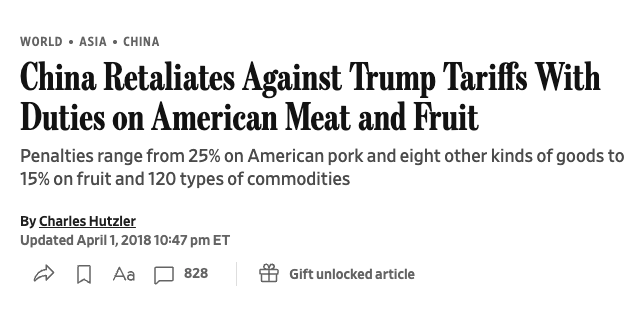
\includegraphics[width=\textwidth, height=5cm, keepaspectratio]{fig/trade_war.png}
    \end{column}
    \begin{column}{0.40\textwidth}
       When the U.S.\ raised tariffs, trading partners hit back.

      \vspace{0.5em}
      American exporters---who had \textit{nothing to do with steel}---paid the price.
    \end{column}
  \end{columns}

\end{frame}

\begin{frame}{Claim 3: Are Tariffs a Good Fix?}
  \centering

  {\Large\textbf{``If international trade is not good for every sector, \underline{tariffs} can protect those affected sectors.''}}

  \vspace{2em}
  \pause
  \begin{answerbox}
    \textbf{It's complicated.} Tariffs can protect specific \textit{sectors}, but they
    raise costs for consumers and downstream firms. The costs often outweigh the
    benefits. Retaliation hurts unrelated industries.
  \end{answerbox}

  \vspace{0.5em}
  \textcolor{DarkGray}{\textit{There is no free lunch---every policy involves tradeoffs.}}

\end{frame}



% =============================================================================
\section{Recap}
% =============================================================================

\begin{frame}{Let's Revisit Our Three Claims}

  \vspace{0.5em}
  \begin{enumerate}
    \item ``International trade is generally good for a country's economy.''\\
          $\rightarrow$ \textcolor{green}{\textbf{Yes}}---comparative advantage grows the pie.

    \vspace{1em}
    \item ``International trade is generally good for every sector of a country's economy.''\\
          $\rightarrow$ \textcolor{vermillion}{\textbf{No}}---creates winners and losers. Transition is hard.

    \vspace{1em}
    \item ``Tariffs protect a country when international trade is bad for the economy.''\\
          $\rightarrow$ \textcolor{orange}{\textbf{It's complicated}}---protects some, taxes others. Costs often exceed benefits.
  \end{enumerate}


\end{frame}

\end{document}
